\documentclass{article}

\usepackage[utf8]{inputenc}
\usepackage[spanish]{babel}
\usepackage[top=2cm,bottom=2cm,right=2.5cm,left=2.5cm]{geometry}
\usepackage{amsmath,amsthm,amssymb}
\usepackage{wrapfig,float,graphicx,parskip,verbatim,multirow,color,minted,listing,multicol}
\begin{document}


\onecolumn\begin{@twocolumntrue}
    \begin{minipage}{0.3\textwidth}{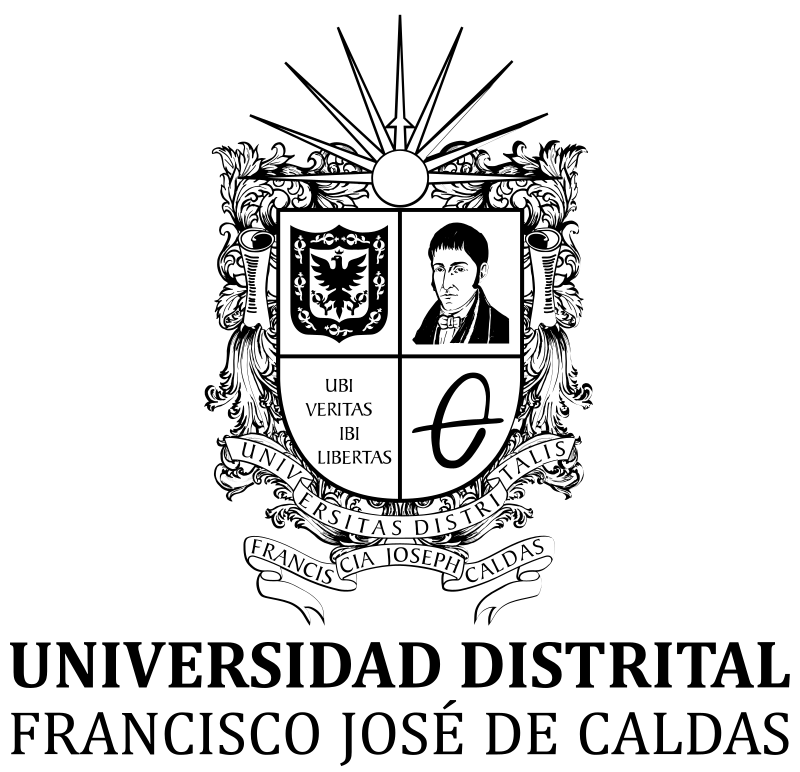
\includegraphics[scale=0.18]{Escudo_UD.svg.png}} % Cambiar escudo
    \end{minipage}
    \vspace{10pt}
    \begin{minipage}{0.677\textwidth}
        \begin{center}
            \vspace{12mm}
        
            \Large{\textbf{<<Título>>}}
            \vspace{3mm}
            
            \large{\textbf{<<Autores>>}}
            \vspace{2mm}
    
            \large{\textit{<<Carrera>>, <<Universidad>>}}
            \vspace{1mm}
            
            <<Fecha>> % Formato (mes) de (año)
        \end{center}
\vspace{5pt}
\end{minipage}

\centerline{\rule{0.95\textwidth}{0.4pt}} % Línea negra
\end{@twocolumntrue}

\begin{center}
    \Large \textbf{Resumen}
    
    \small
    <<Texto>>
\end{center}
\hspace{10pt}\textbf{Palabras clave:} <<Texto>>
\begin{center}
    \Large \textbf{Abstract}
    
    \small
    <<Text>>
\end{center}
\hspace{10pt}\textbf{Keywords:} <<Text>>

\centerline{\rule{0.95\textwidth}{0.4pt}}
\vspace{15pt}

\begin{multicols}{2}

\section{Introducción}

<<Texto>>

\section{Sección 1} 

\begin{equation}
    Ecuaciones
\label{ecuacion}
\end{equation}

\begin{equation*} % Para ecuaciones sin número y que el igual se mantenga en la misma sangría
\begin{split}
    texto1 & = texto---2 \\
    texto---2 & = texto------3 \\
    texto------3 & = texto4
\end{split}
\end{equation*}

\section{Sección 2}

<<Texto>>

\end{multicols}

\subsection{Subsección 1}

<<Variación entre dos y una columna>> -------------------------------------------------------------------

\begin{multicols}{2}

\subsection{Subsección 2}

<<Texto>>

\subsubsection{Subsubsección 1}

<<Texto>>

\begin{figure}[H]
    \centering
    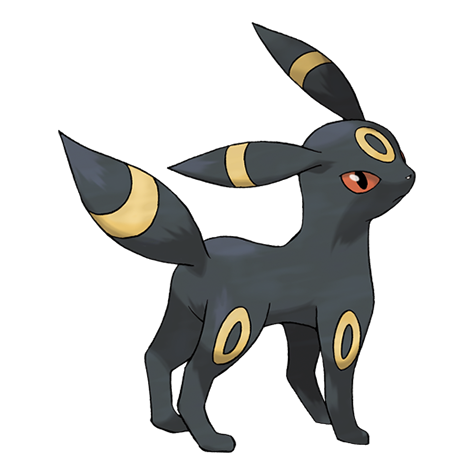
\includegraphics[scale=0.32]{pollito.png}
    \caption{Inserción de una figura}
    \label{figura}
\end{figure}

\section{Conclusiones}

<<Conclusión>>

\section{Bibliografía}

[1] <<Referencia>>

\end{multicols}

\section{Anexos}

<<Anexo>>

\end{document}